\documentclass[12pt]{article}
\usepackage{graphicx}
\usepackage{geometry}
\usepackage{pdfpages}
\usepackage{titlesec}
\usepackage{centernot}
\usepackage{fancyhdr}
\usepackage{hyperref}
% Margins
\geometry{
    a4paper,
    total={170mm,257mm},
    left=20mm,
    top=20mm,
}

\begin{document}

% Title page
\begin{titlepage}
    \centering
    \vspace*{5cm}
    
    {\Huge \textbf{MEC6602E: Transonic Aerodynamics}}\\[1.5cm]
    
    {\Large \textbf{HOMEWORK 1}}\\[2cm]
    
    {\Large Prepared by:}\\
    {\Large Kamal Jemmali 2019339}\\
    {\Large Hugo Javourez 2420717}\\[1.5cm]
    
    {\Large Submitted to :}\\
    {\Large M.Frédéric Plante. Ph.D, CPI}\\[2cm]
    
    {\Large Due date :}\\
    {\Large 24 september 2024}\\
    
    \vfill
    
\includegraphics[width=0.25\textwidth]{polytechnique-signature-rgb-gauche-fr.png} % Placeholder for a logo or image (optional)
    
    \vfill
\end{titlepage}

% Title of the section
\section{Question 1: Analytical Calculation of Order of Convergence, Stability and Consistency}

This section will analyse some finite difference algorithms of the following equation:
\begin{equation}
    \frac{\partial u}{\partial t} + c \frac{\partial u}{\partial x} = 0
\end{equation}

This will be done by 3 ways:

\begin{itemize}
    \item Analysing convergence with Taylor
    \item Stability with Von Neumann
    \item Consistensy with le limit of the error term $\Delta x, \Delta t \longrightarrow 0$ \\[1cm]
\end{itemize}



a1. Lets analyse the backward algorithm:
\begin{equation}
    u_j^{n+1} = u_j^n - \frac{c \Delta t}{\Delta x} \left( u_j^n - u_{j-1}^n \right)
\end{equation}

This Algorithm is:

\begin{itemize}
    \item Stable
    \item Convergent on ordre 1 in both time and space
    \item Consistent\\[1cm]
\end{itemize}


a2. Lets analyse the frontward algorithm:
\begin{equation}
    u_j^{n+1} = u_j^n - \frac{c \Delta t}{\Delta x} \left( u_{j+1}^n - u_{j}^n \right)
\end{equation}

This Algorithm is:

\begin{itemize}
    \item UnStable
    \item Convergent on ordre 1 in both time and space
    \item Consistent\\[1cm]
\end{itemize}

b. Lets analyse the centered algorithm:
\begin{equation}
    u_j^{n+1} = u_j^n - \frac{c \Delta t}{\Delta x} \left( u_{j+1}^n - u_{j-1}^n \right)
\end{equation}

This Algorithm is:

\begin{itemize}
    \item UnStable
    \item Convergent on ordre 2 in space and ordre 1 in time 
    \item Consistent\\[1cm]
\end{itemize}

c. Lets analyse the leap-frog algorithm:
\begin{equation}
    u_j^{n+1} = u_j^{n-1} - \frac{c \Delta t}{\Delta x} \left( u_{j+1}^n - u_{j-1}^n \right)
\end{equation}

This Algorithm is:

\begin{itemize}
    \item Metastable $|G| = 1$
    \item Convergent on ordre 2 in space and ordre 2 in time 
    \item Consistent\\[1cm]
\end{itemize}

d. Lets analyse the Lax-Wendroff algorithm:
\begin{equation}
    u_j^{n+1} = u_j^n - \frac{c \Delta t}{2 \Delta x} \left( u_{j+1}^n - u_{j-1}^n \right)
+ \frac{1}{2} \left( \frac{c \Delta t}{\Delta x} \right)^2 \left( u_{j+1}^n - 2 u_j^n + u_{j-1}^n \right)
\end{equation}

This Algorithm is:

\begin{itemize}
    \item Stable $CFL<1$
    \item Convergent on ordre 2 in space and ordre 1 in time 
    \item Consistent\\[1cm]
\end{itemize}

e. Lets analyse the Lax algorithm:
\begin{equation}
    u_j^{n+1} = u_j^n - \frac{c \Delta t}{2 \Delta x} \left( u_{j+1}^n - u_{j-1}^n \right)
+ \frac{1}{2} \left( \frac{c \Delta t}{\Delta x} \right)^2 \left( u_{j+1}^n - 2 u_j^n + u_{j-1}^n \right)
\end{equation}

This Algorithm is:

\begin{itemize}
    \item Stable $CFL<1$
    \item Bad convergence and not consistent\\[1cm]
\end{itemize}

f. Lets analyse the Hybrid algorithm:

For $\theta = 0$ This Algorithm is:

\begin{itemize}
    \item the same as the b, please refer to it \\[1cm]
\end{itemize}

For $\theta = 1$ This Algorithm is:

\begin{itemize}
    \item Always Stable
    \item first ordre in time, 2nd order in space
    \item consistent \\[1cm]
\end{itemize}

For $\theta = 0.5$ This Algorithm is:

\begin{itemize}
    \item Metastable $|G| = 1$
    \item first ordre in time, 2nd order in space
    \item consistent \\[1cm]
\end{itemize}

g. Lets Analyse our chosen algorithm:

Here are the 2th order in space discretisation and the 4th order in time chosen:

\begin{equation}
    \frac{\partial u}{\partial x} \approx \frac{u_{j+1}^n - u_{j-1}^n}{2 \Delta x}
\end{equation}

\begin{equation}
    \frac{\partial u}{\partial t} \approx \frac{- u_j^{n+2} + 8 u_j^{n+1} - 8 u_j^{n-1} + u_j^{n-2}}{12 \Delta t}
\end{equation}

\begin{equation}
    u_j^{n+1} = \frac{1}{8} u_j^{n+2} + u_{j}^{n-1} - \frac{1}{8} u_{j}^{n-2}
    -\frac{3c \Delta t}{4 \Delta x} \left( u_{j+1}^{n} - u_{j-1}^{n} \right)
\end{equation}

\begin{itemize}
    \item Unstable
    \item 4nd order in time, 2nd order in space
    \item Consistent \\[1cm]
\end{itemize}

Of course, every calculation will be found on the annexe 1

\newpage
\section{NUMERICAL ANALYSIS}


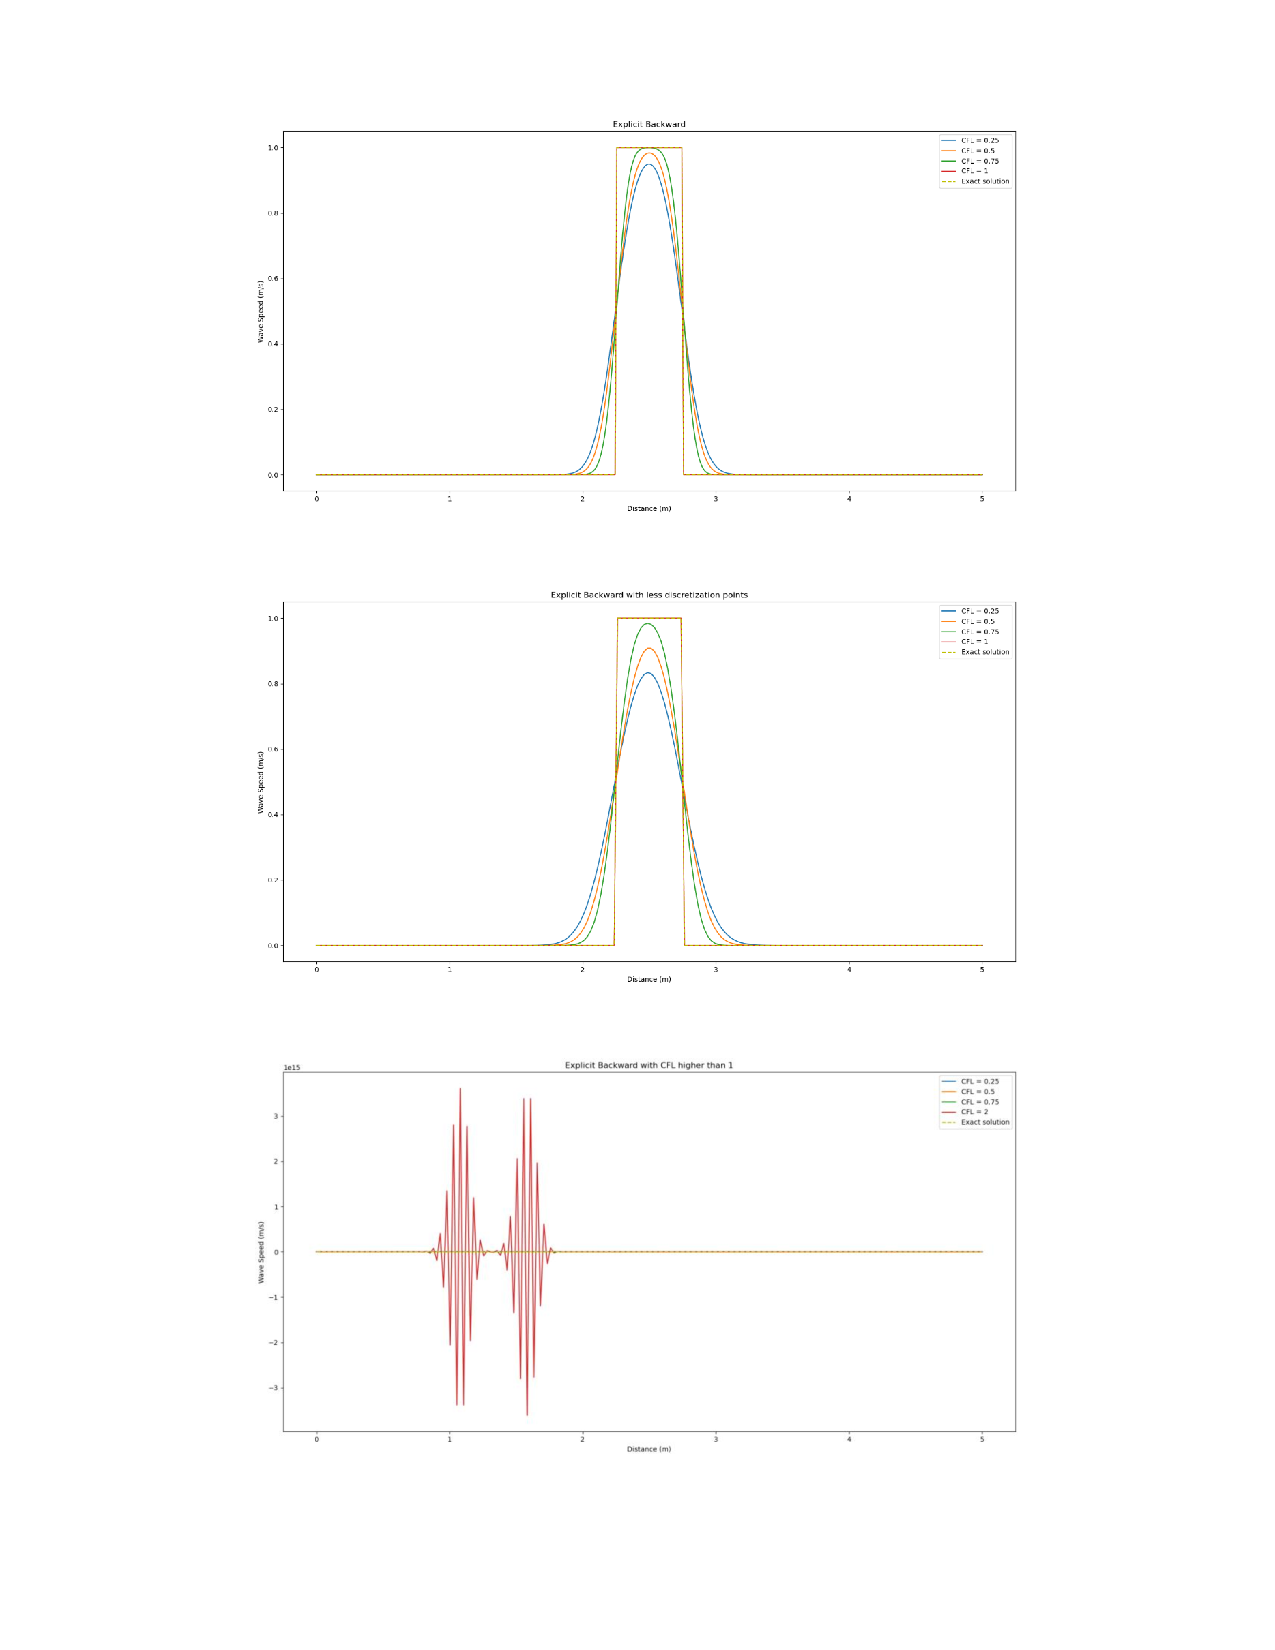
\includepdf[pages=-]{Numerical analysis comments.pdf}




\newpage

\section{ANNEXE 1}
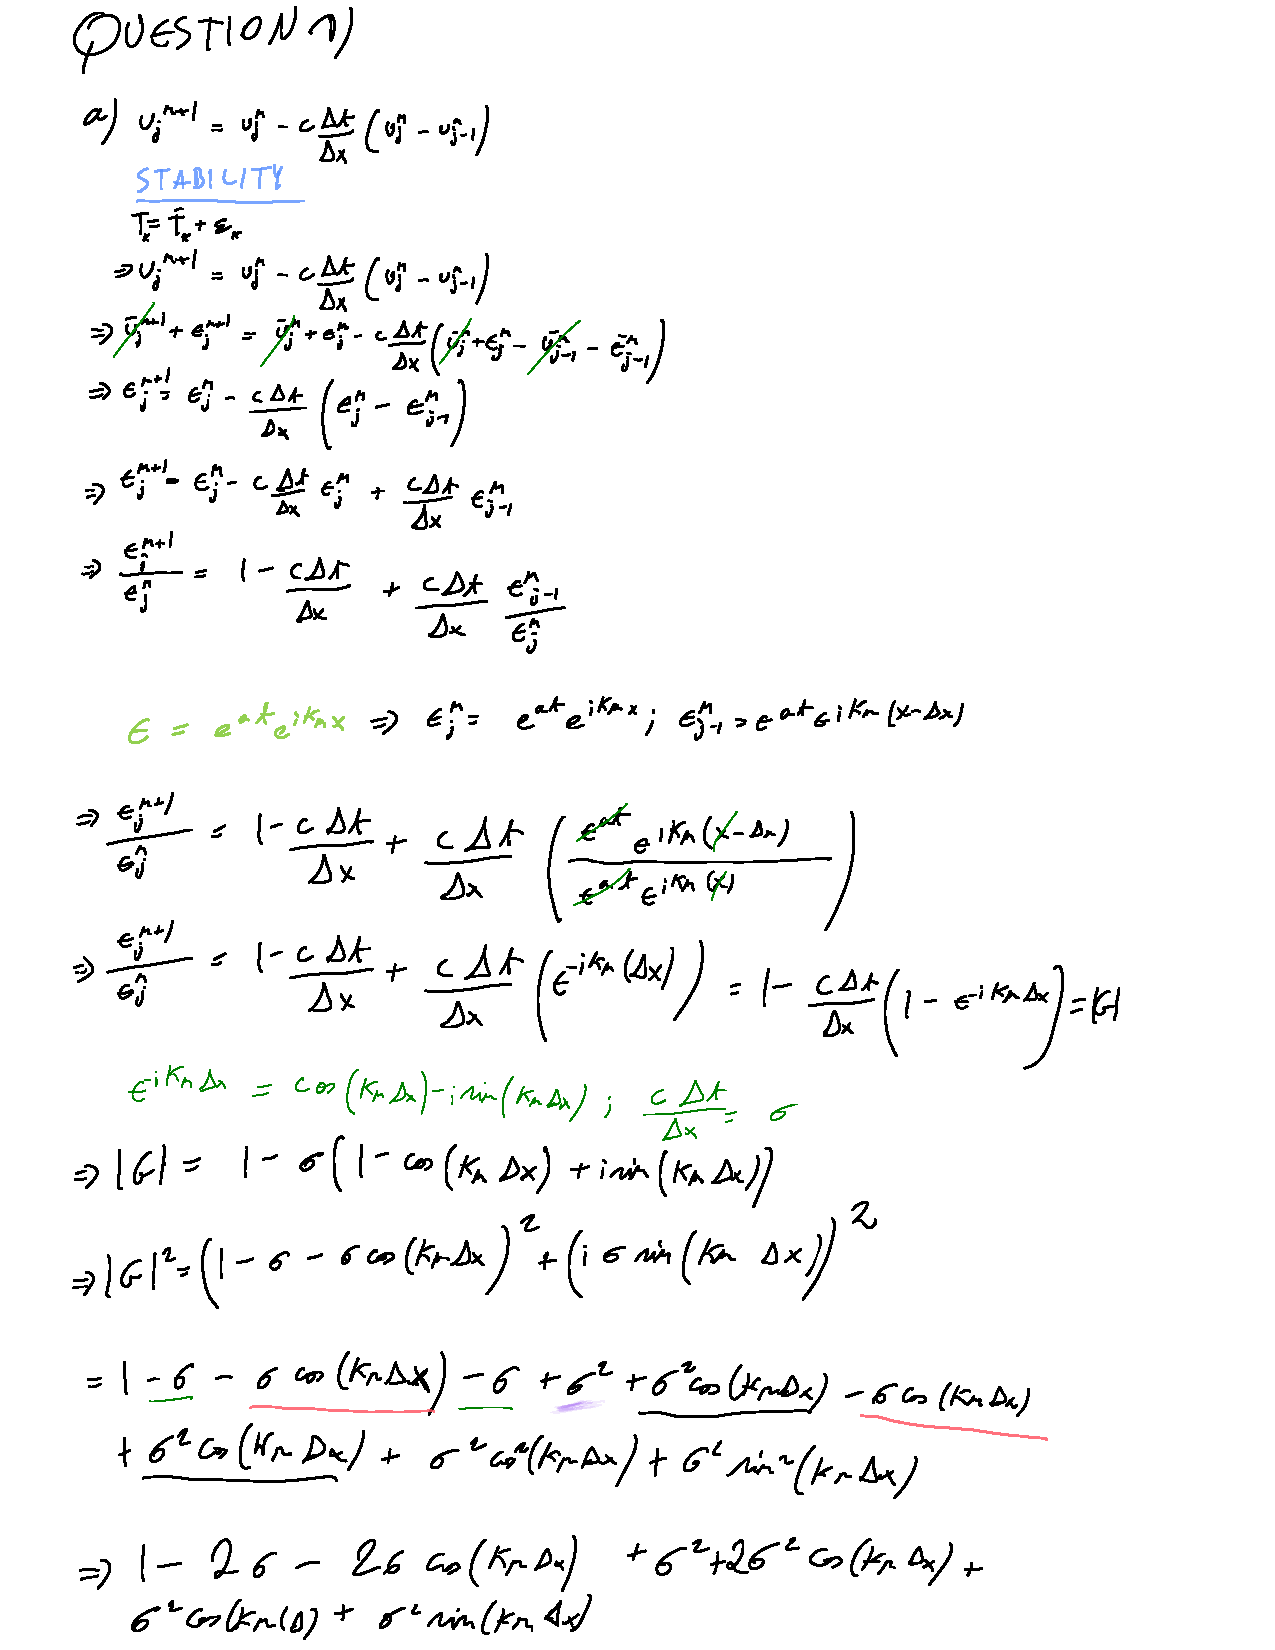
\includepdf[pages=-]{question 1a lite.pdf}
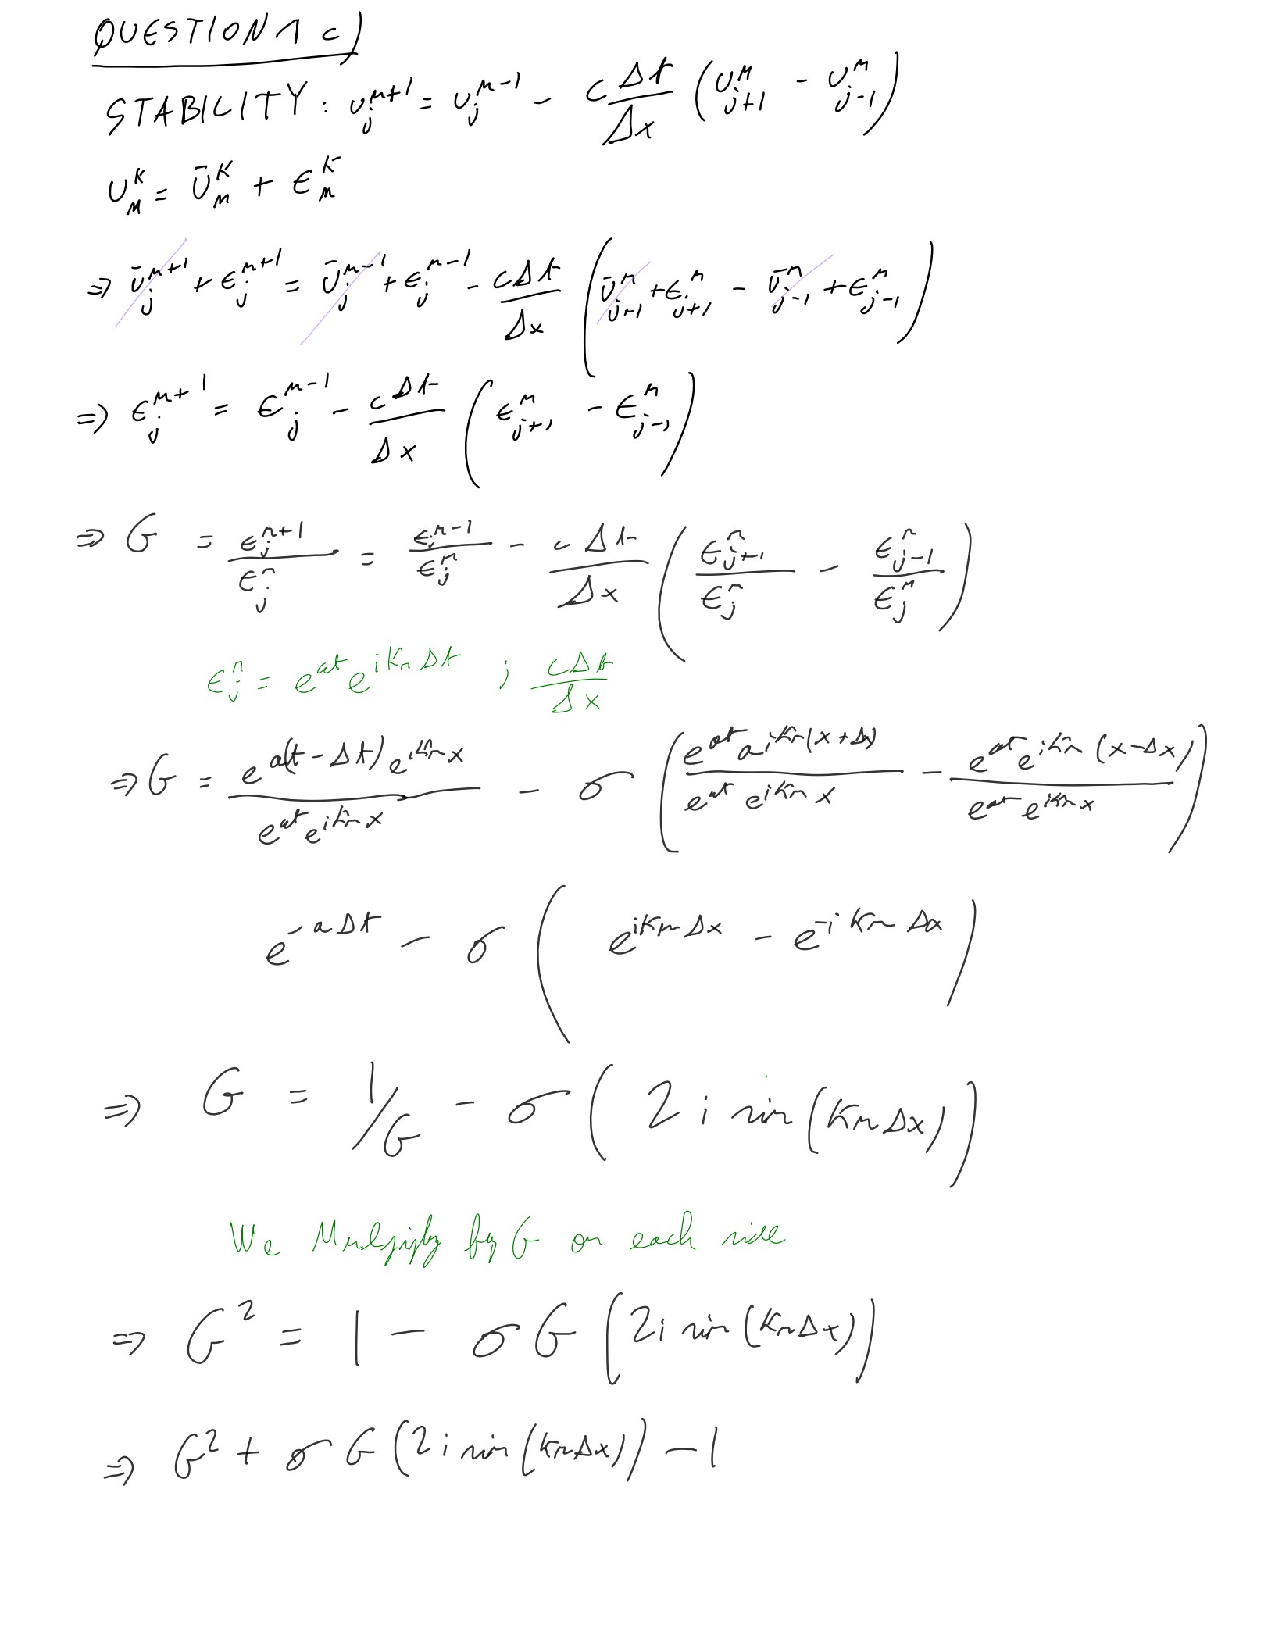
\includepdf[pages=-]{question 1c lite.pdf}
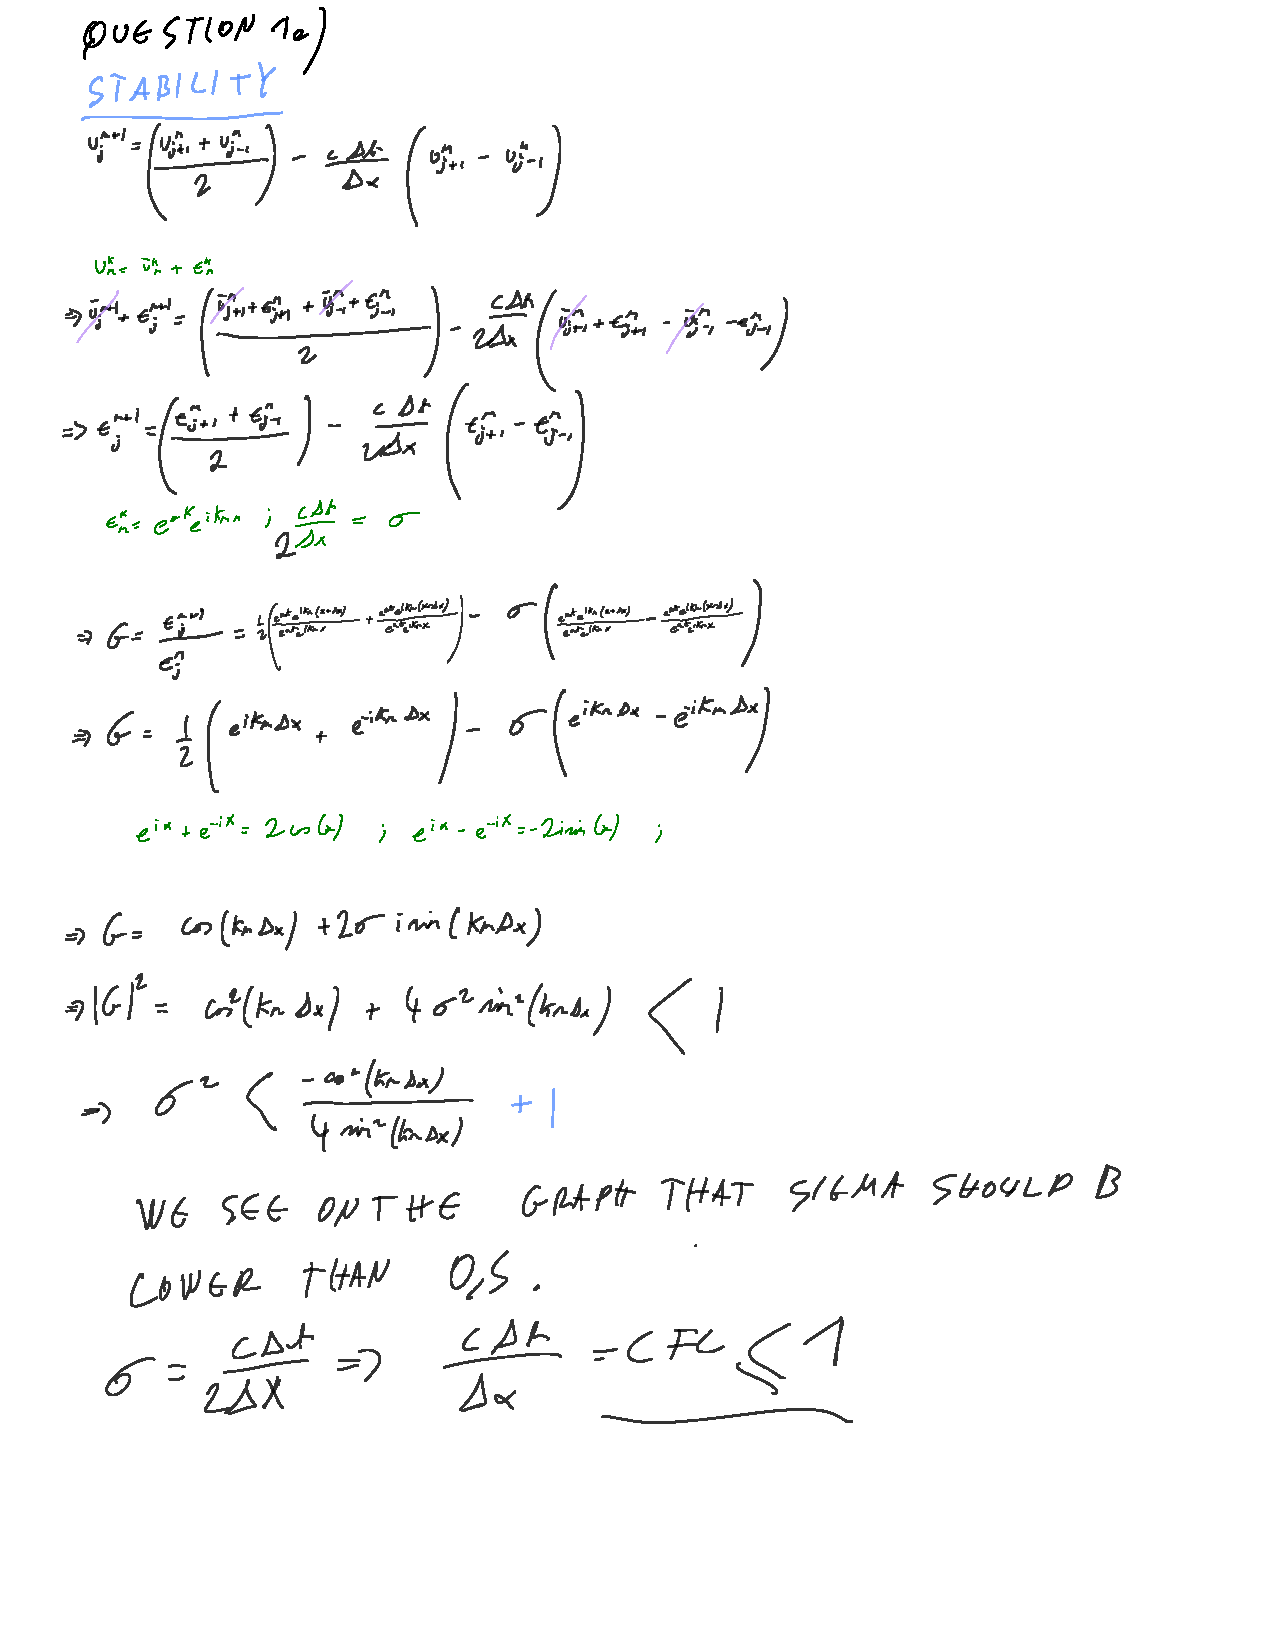
\includepdf[pages=-]{question 1e lite.pdf}
\includepdf[pages=-]{question 1g lite.pdf}
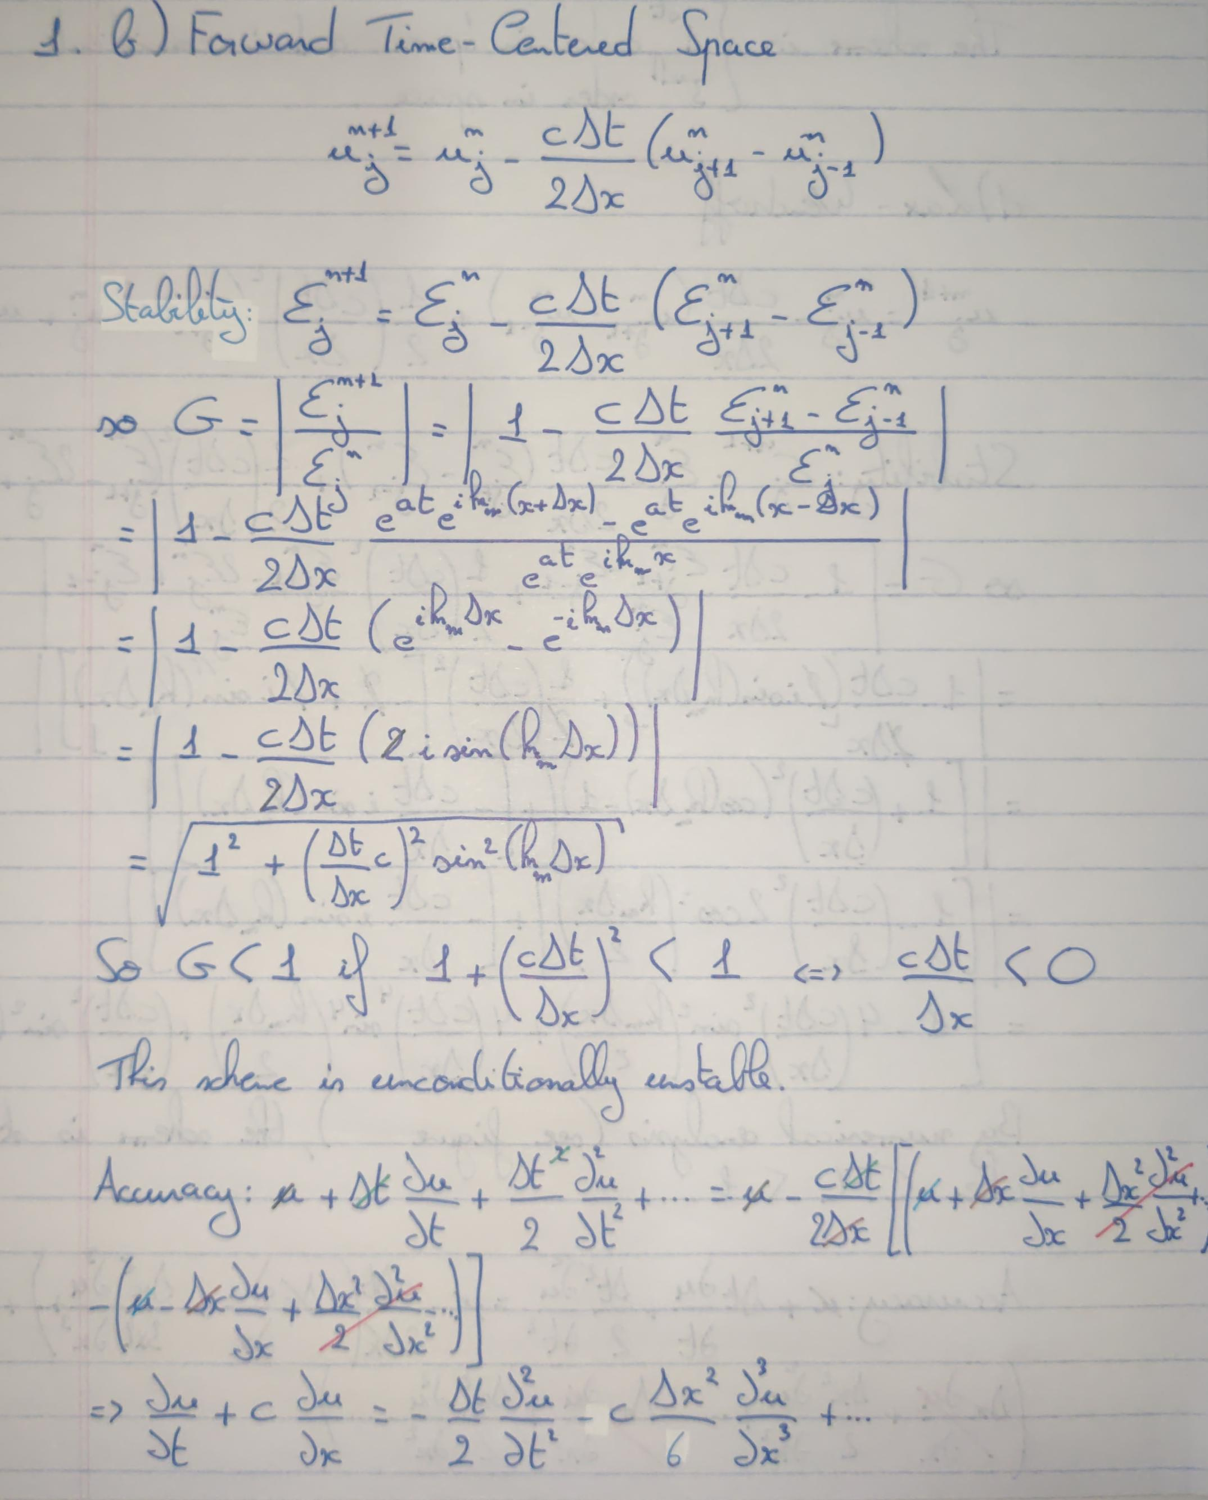
\includepdf[pages=-]{Question b and d}
\vfill
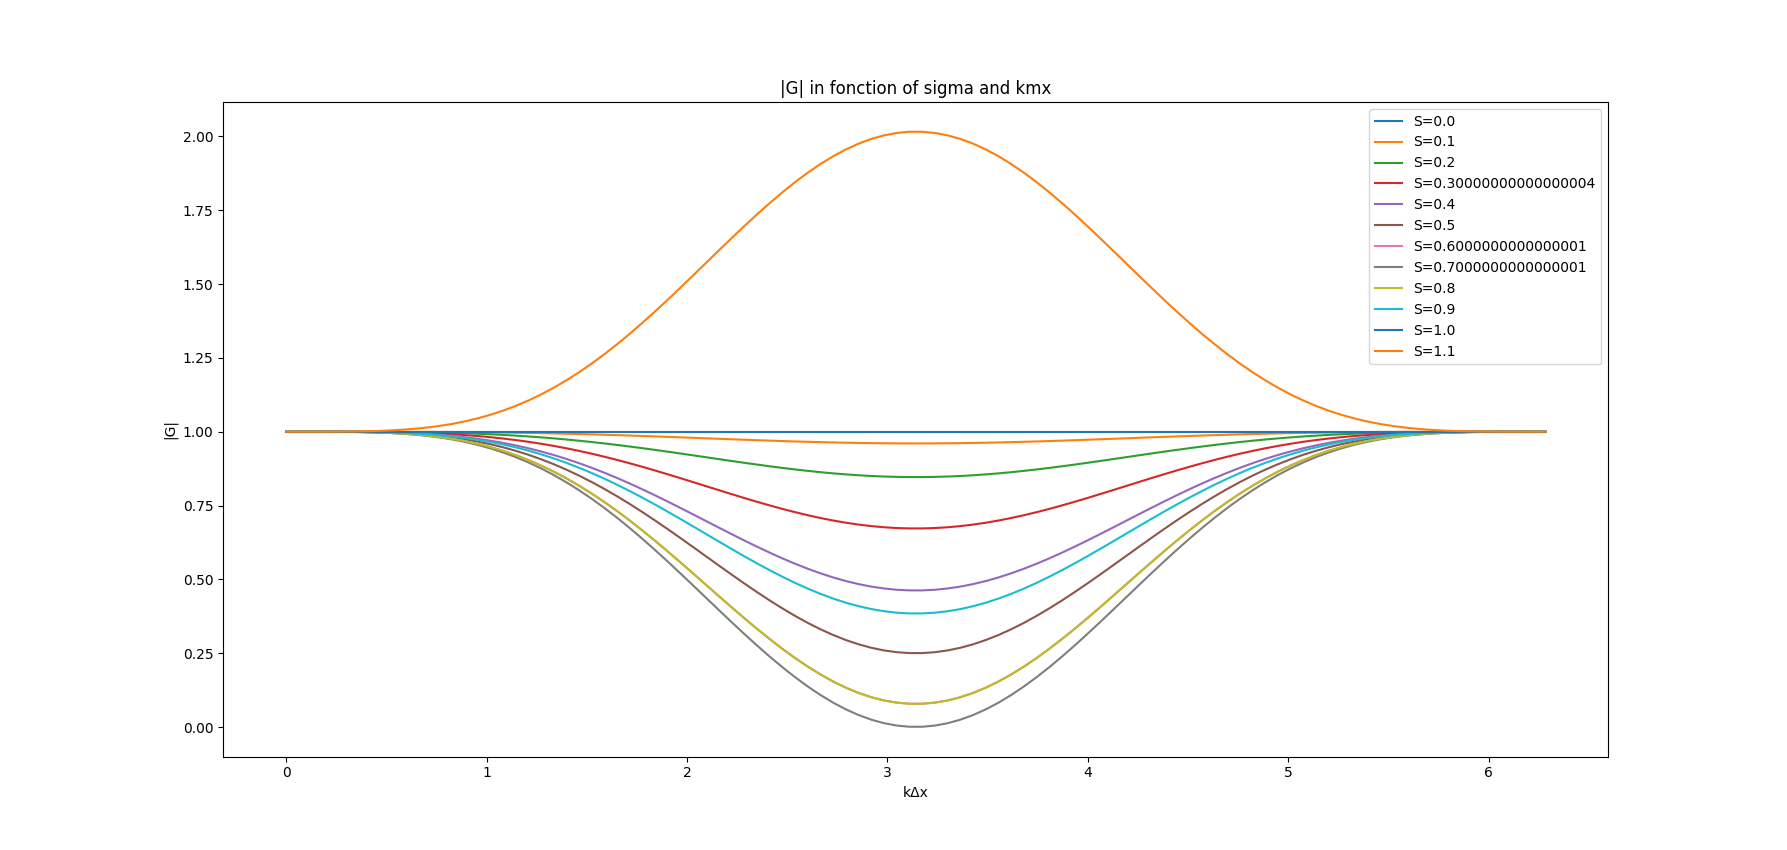
\includegraphics[width=1\textwidth]{sigma_question d.png}
\vfill
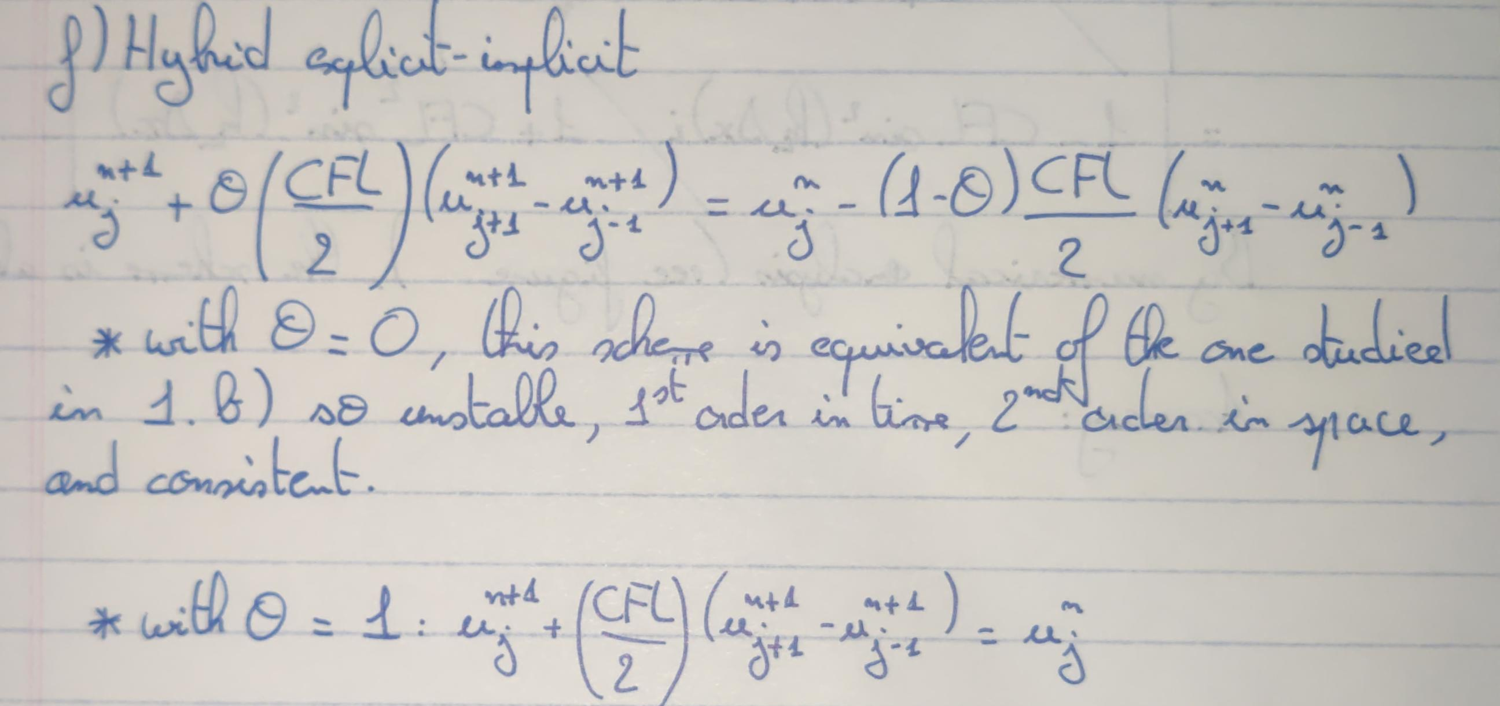
\includepdf[pages=-]{Question f 0 and 1}
\vfill
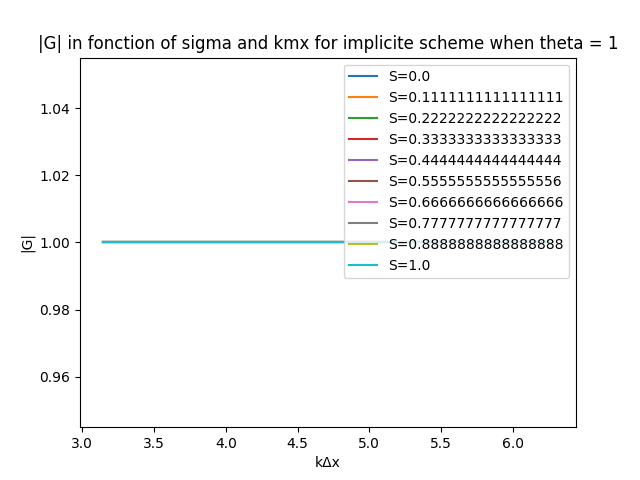
\includegraphics[width=1\textwidth]{sigma_f_1.png}
\vfill
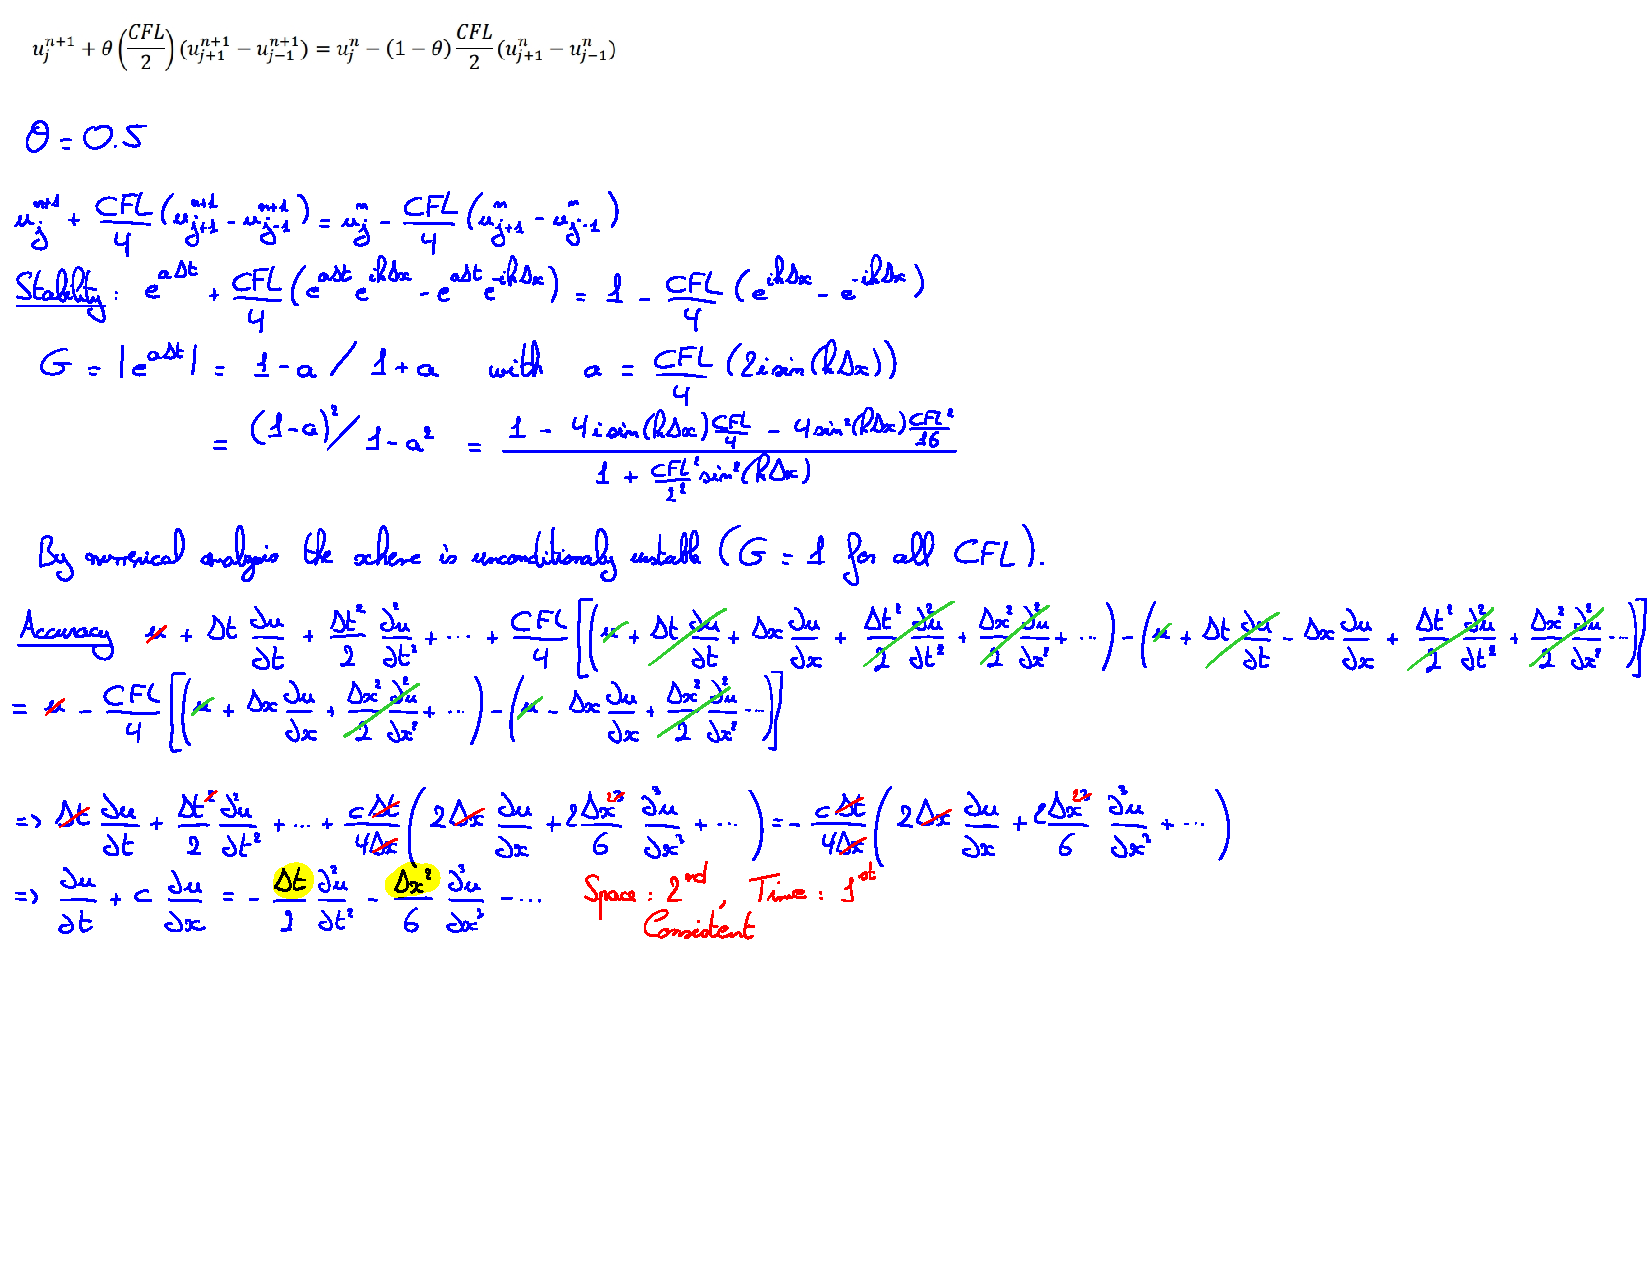
\includepdf[pages=-]{Question f 0.5}
\vfill
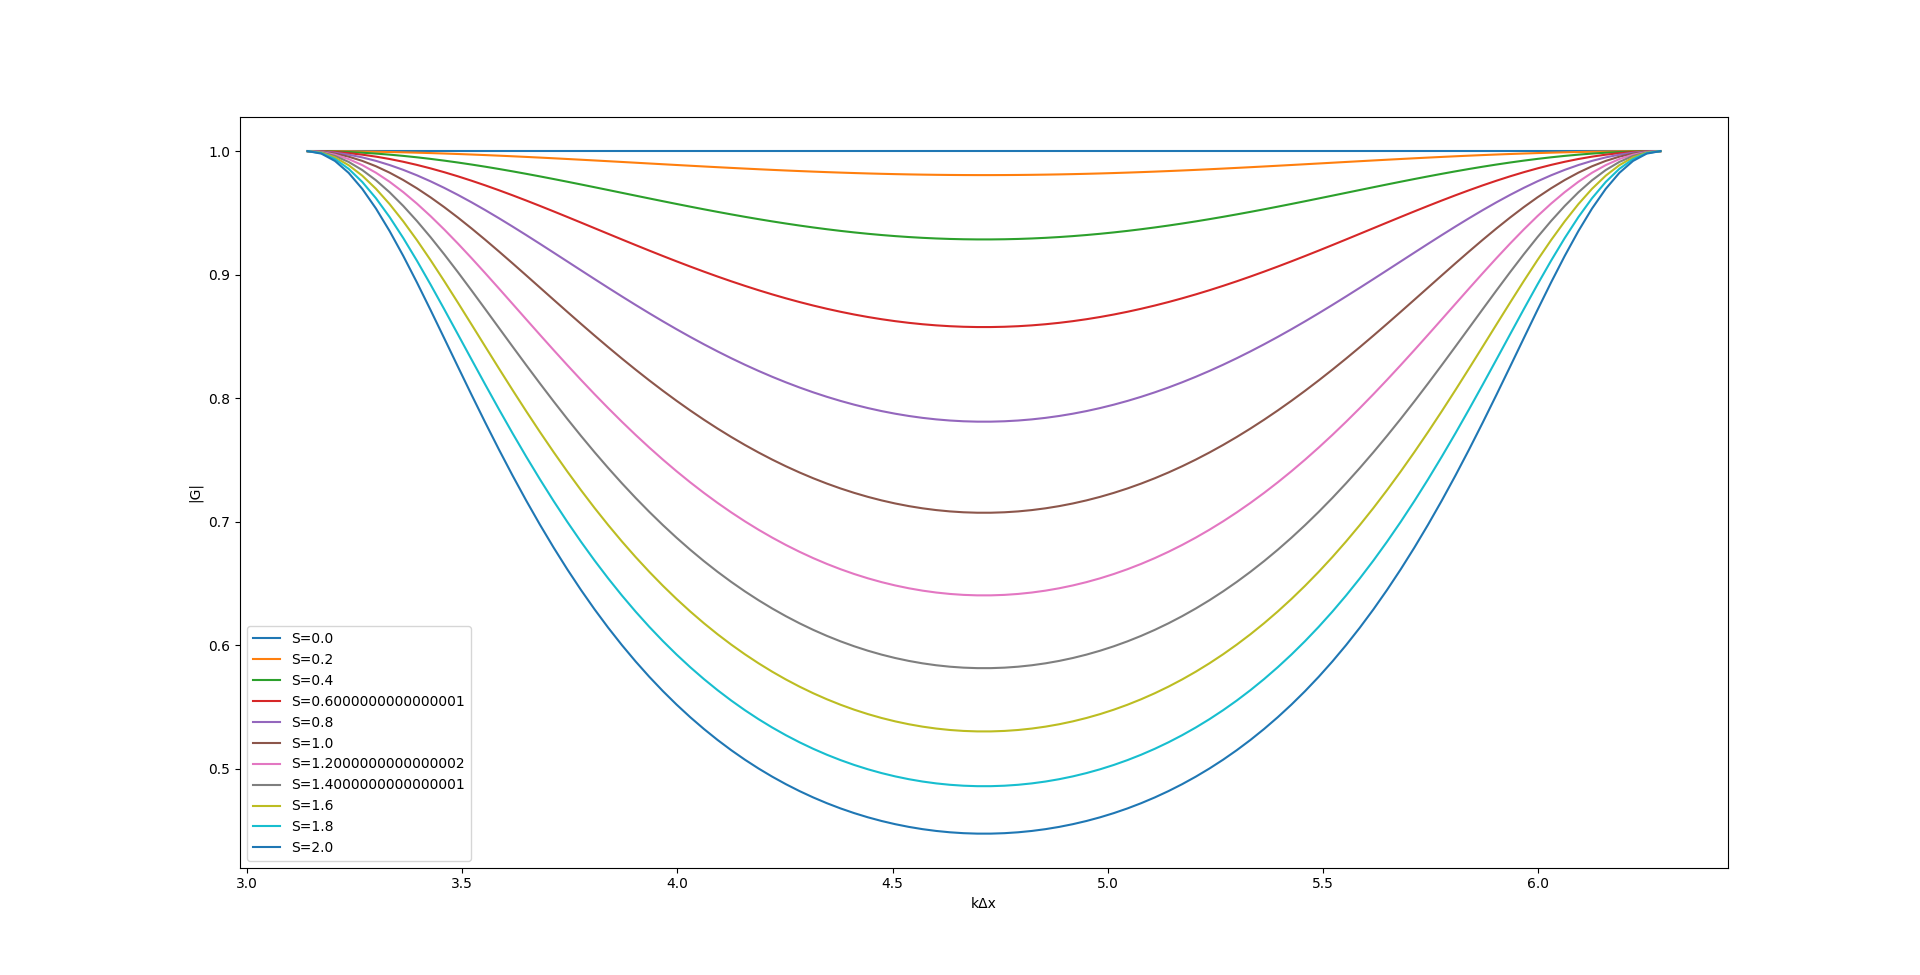
\includegraphics[width=1\textwidth]{sigma_f_05.png}
\vfill

\section{ANNEXE 2: GITHUB LINK}

\href{https://github.com/Kenesis69/MEC_6602E_HOMEWORK_1}{Cliquez !!! Lien github !!!}

\end{document}
